TO BE DONE:
\bn

\item Implement above algorithm

\item Select case studies. We need examples that have ``branching
waiting'' behavior, \ie a process waits for alternatives. For example,
dining philosopher is NOT an example of this. 

One possible source is the paper 
``Evaluating Deadlock Detection Methods for Concurrent Software'', 
IEEE Transactions on Software Engineering, Vol. 22, No. 3, March 1996

\en




\subsubsection{Experiment: Dining Philosophers} 
We consider $n$ philosophers in a cycle, based on the components of Figure~\ref{fig:diningSpectrum}.
Figure~\ref{bench:dining} provides experimental results.
The $x$ axis gives the number $n$ of philosophers (and also the number of forks), 
and the $y$ axis gives the verification time (in
milliseconds).  We verified that $\LDFC(a, \l)$ holds for
$\l = 1$ and all interactions $a$. Hence dining philosophers is deadlock-free.
%
We increase $n$ and plot the verification
time for both \ldfctool and D-Finder 2~\cite{DFinder2}.
D-Finder 2 implements a compositional and incremental method for the
verification of BIP-systems. D-Finder
(the precursor of D-Finder 2) has been compared favorably with NuSmv and
SPIN, outperforming both  NuSmv and SPIN on
dining philosophers, and outperforming NuSmv on the gas station
example~\cite{bensalem2010compositional}, treated next.
%
Our results show that \ldfctool has a linear increase of computation time with the system size
$(n)$, and so outperforms D-Finder 2.


\subsubsection{Experiment: Gas Station}
A gas station \cite{gasstation} consists of an operator, % with a computer,
a set of pumps, and a set of customers. 
%Each pump can be used by a fixed number of customers.
Before using a pump, a customer has to prepay. Then the customer uses the
pump, collects his change and %goes to a state from which he may start
starts a new transaction.
%
Before being used by a customer, a pump has to be activated by the
operator.  When a pump is shut off, it can be re-activated for the
next operation.  


Figure \ref{fig:gas-station} gives the model for a
gas station system for one pump and two customers.  The operator has
two control locations and three ports. The transition labeled with
$\mathit{prepay}$ accepts a customer's prepay and activates the pump for the
customer. When a customer is served, the transition labeled with
$\mathit{finish}$ synchronizes the pump and the customer.  A pump has three
control locations and three ports. Besides the synchronization between
the operator and customer through activate and finish ports, a pump
and a customer are synchronized through $\mathit{start}$ ports.

\begin{figure}[ht]
\begin{center}
\scalebox{0.5}{\input{figs/gas_station.pdf_t}}
\caption{Sketch of Gas Station}
\label{fig:gas-station}
\end{center}
\end{figure}


We verified $\LDFC(\B, Q_0, \act, \l)$ for $\l=2$ and all interactions $a$.
Hence gas station is deadlock-free.  Figures~\ref{bench:gasstation1},
\ref{bench:gasstation2}, and \ref{bench:gasstation3} present the verification
times using \ldfctool and D-Finder 2. We consider a system with 3 pumps and variable number
of customers.  In these figures, the $x$ axis gives the number $n$ of
customers, and the $y$ axis gives the verification time (in seconds).
%
D-Finder 2 suffers state-explosion at $n = 1800$,
because we consider only three pumps, and so the incremental method used by
D-Finder 2 deteriorates. \ldfctool outperforms D-Finder 2 as the number of
customers increases.


\begin{figure}[t]
  \begin{center}
    \mbox{
       \hspace*{-0.5cm}\subfigure[Dining philosophers benchmark.]{\label{bench:dining}\scalebox{0.24}{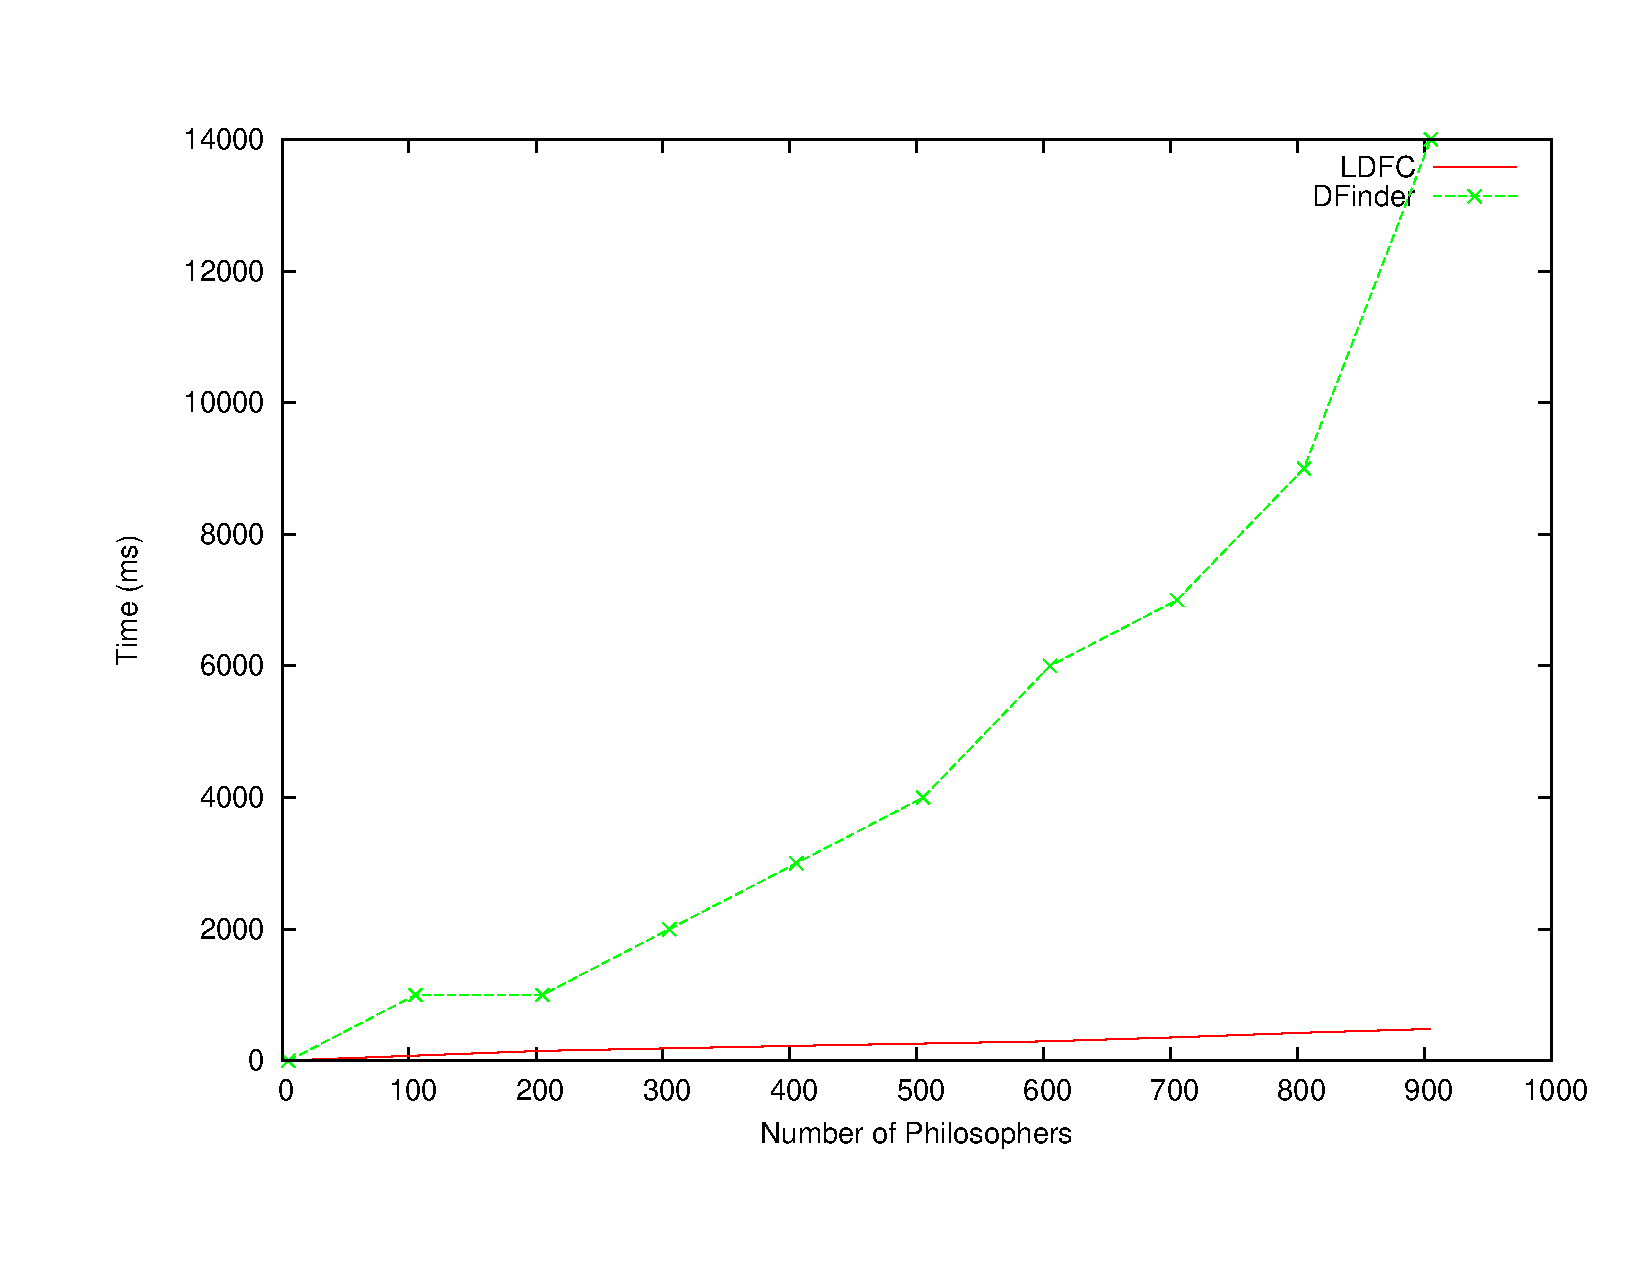
\includegraphics{figs/bench.pdf}}} 
       \hspace*{-0.7cm}\subfigure[Gas station benchmark 1.]{\label{bench:gasstation1}\scalebox{0.24}{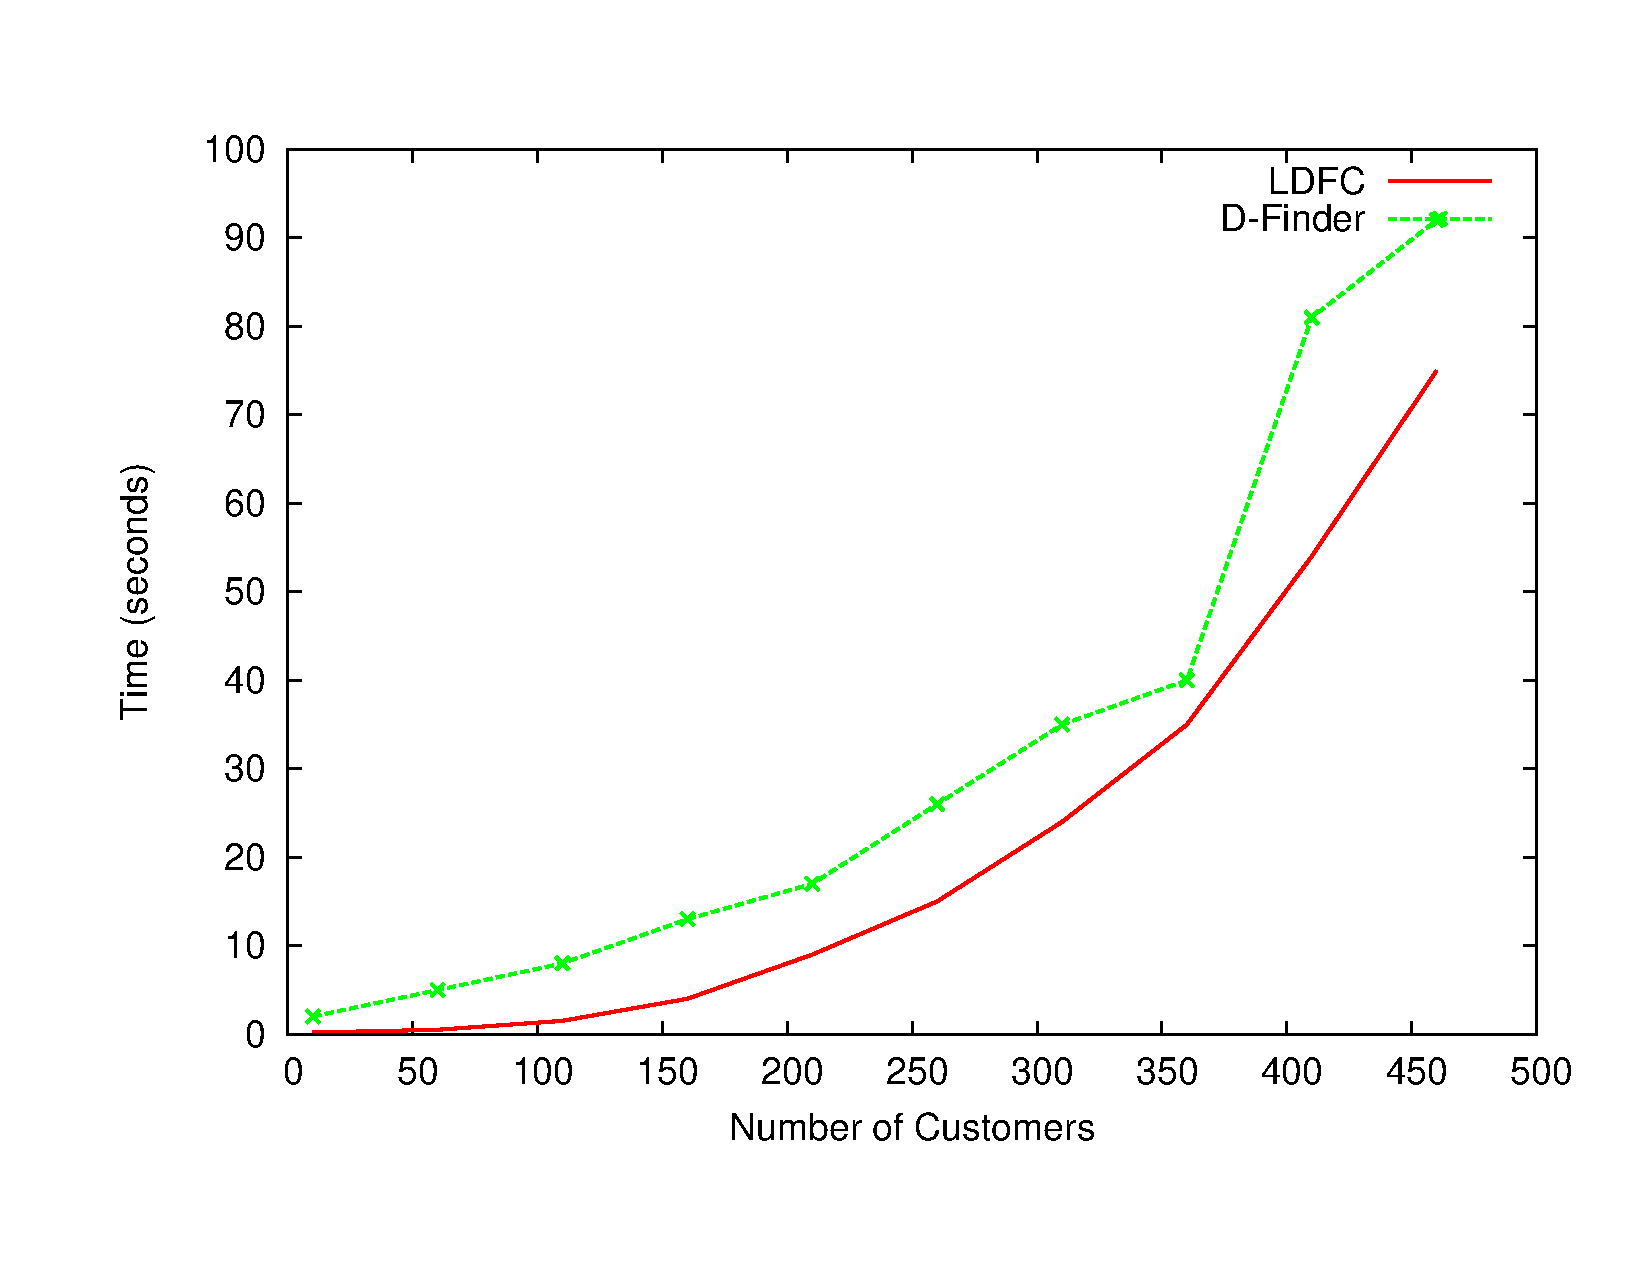
\includegraphics{figs/benchgas1.pdf}}} 
      }\vspace*{0.05cm}
     \mbox{
        \hspace*{-0.6cm} \subfigure[Gas station benchmark 2.]{\label{bench:gasstation2}\scalebox{0.24}{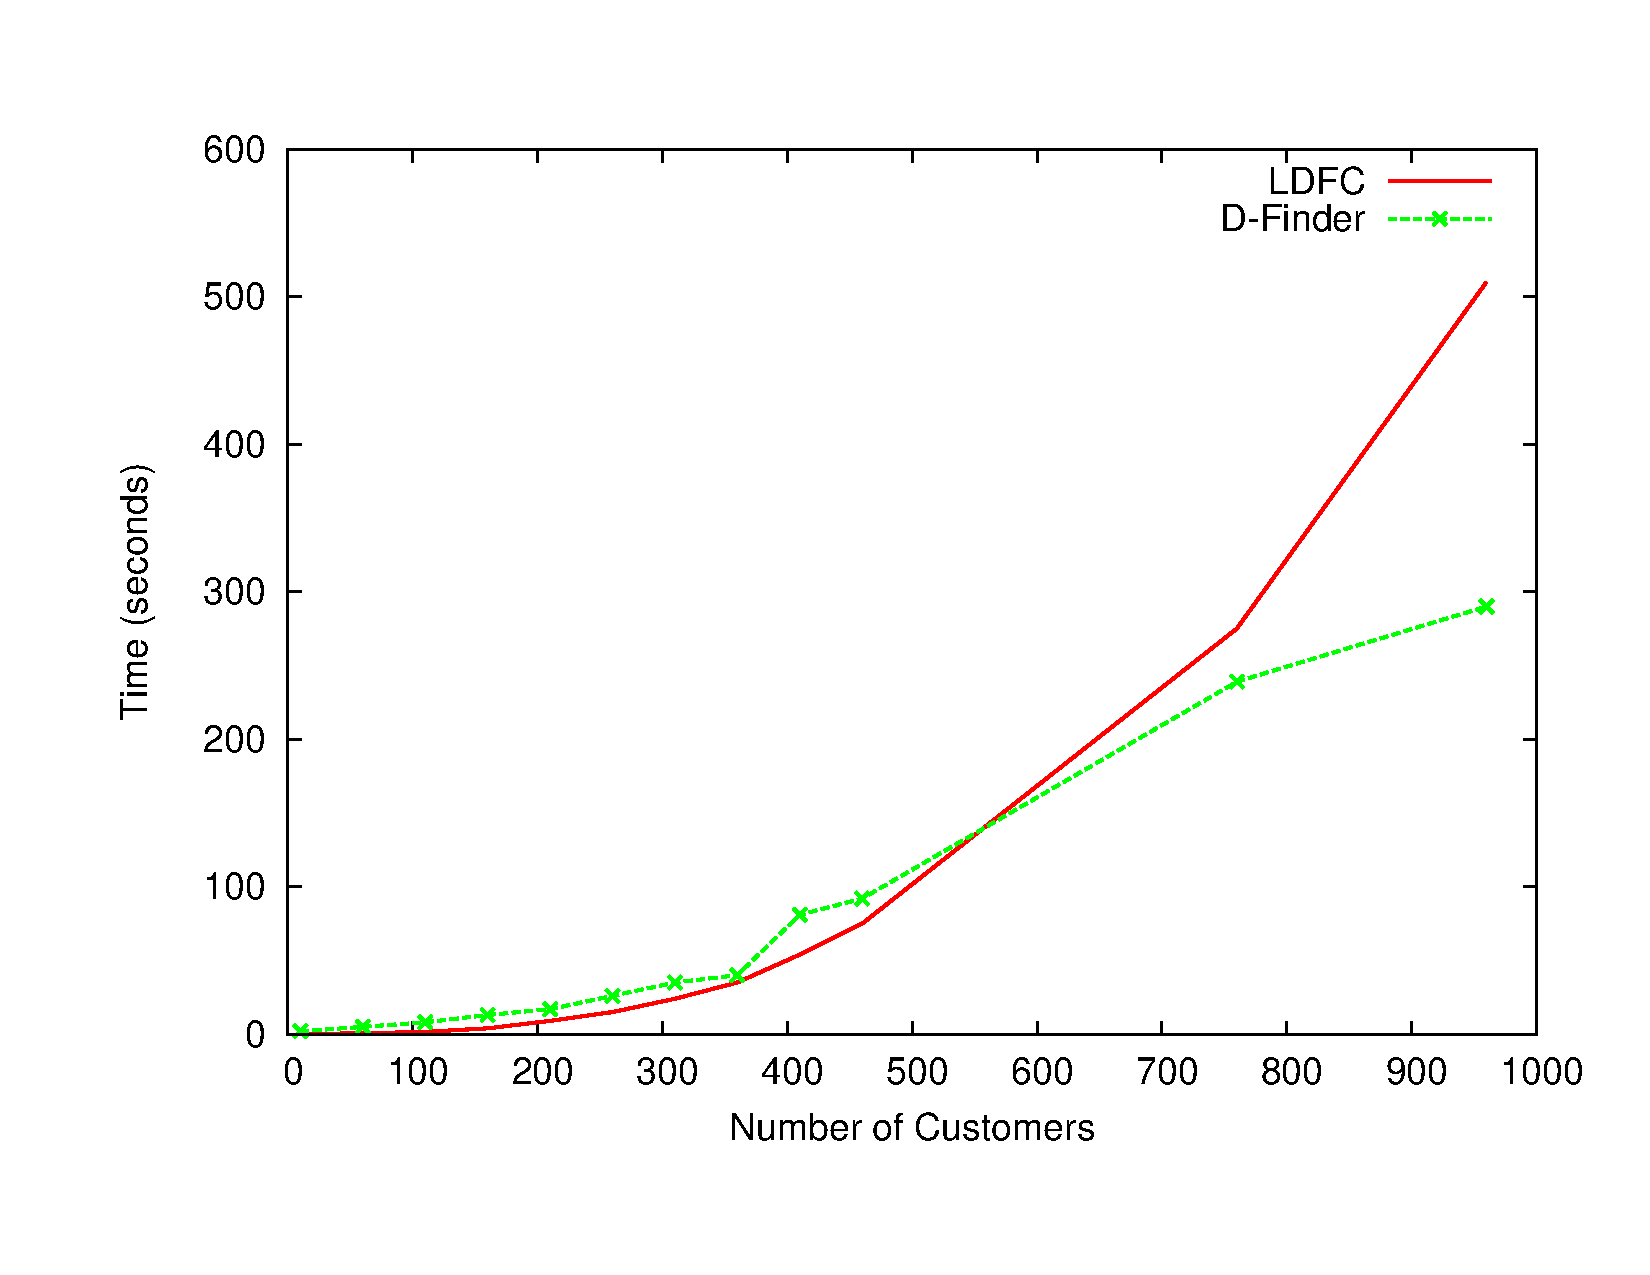
\includegraphics{figs/benchgas2.pdf}}} 
        \hspace*{-0.7cm} \subfigure[Gas station benchmark 3.]{\label{bench:gasstation3}\scalebox{0.24}{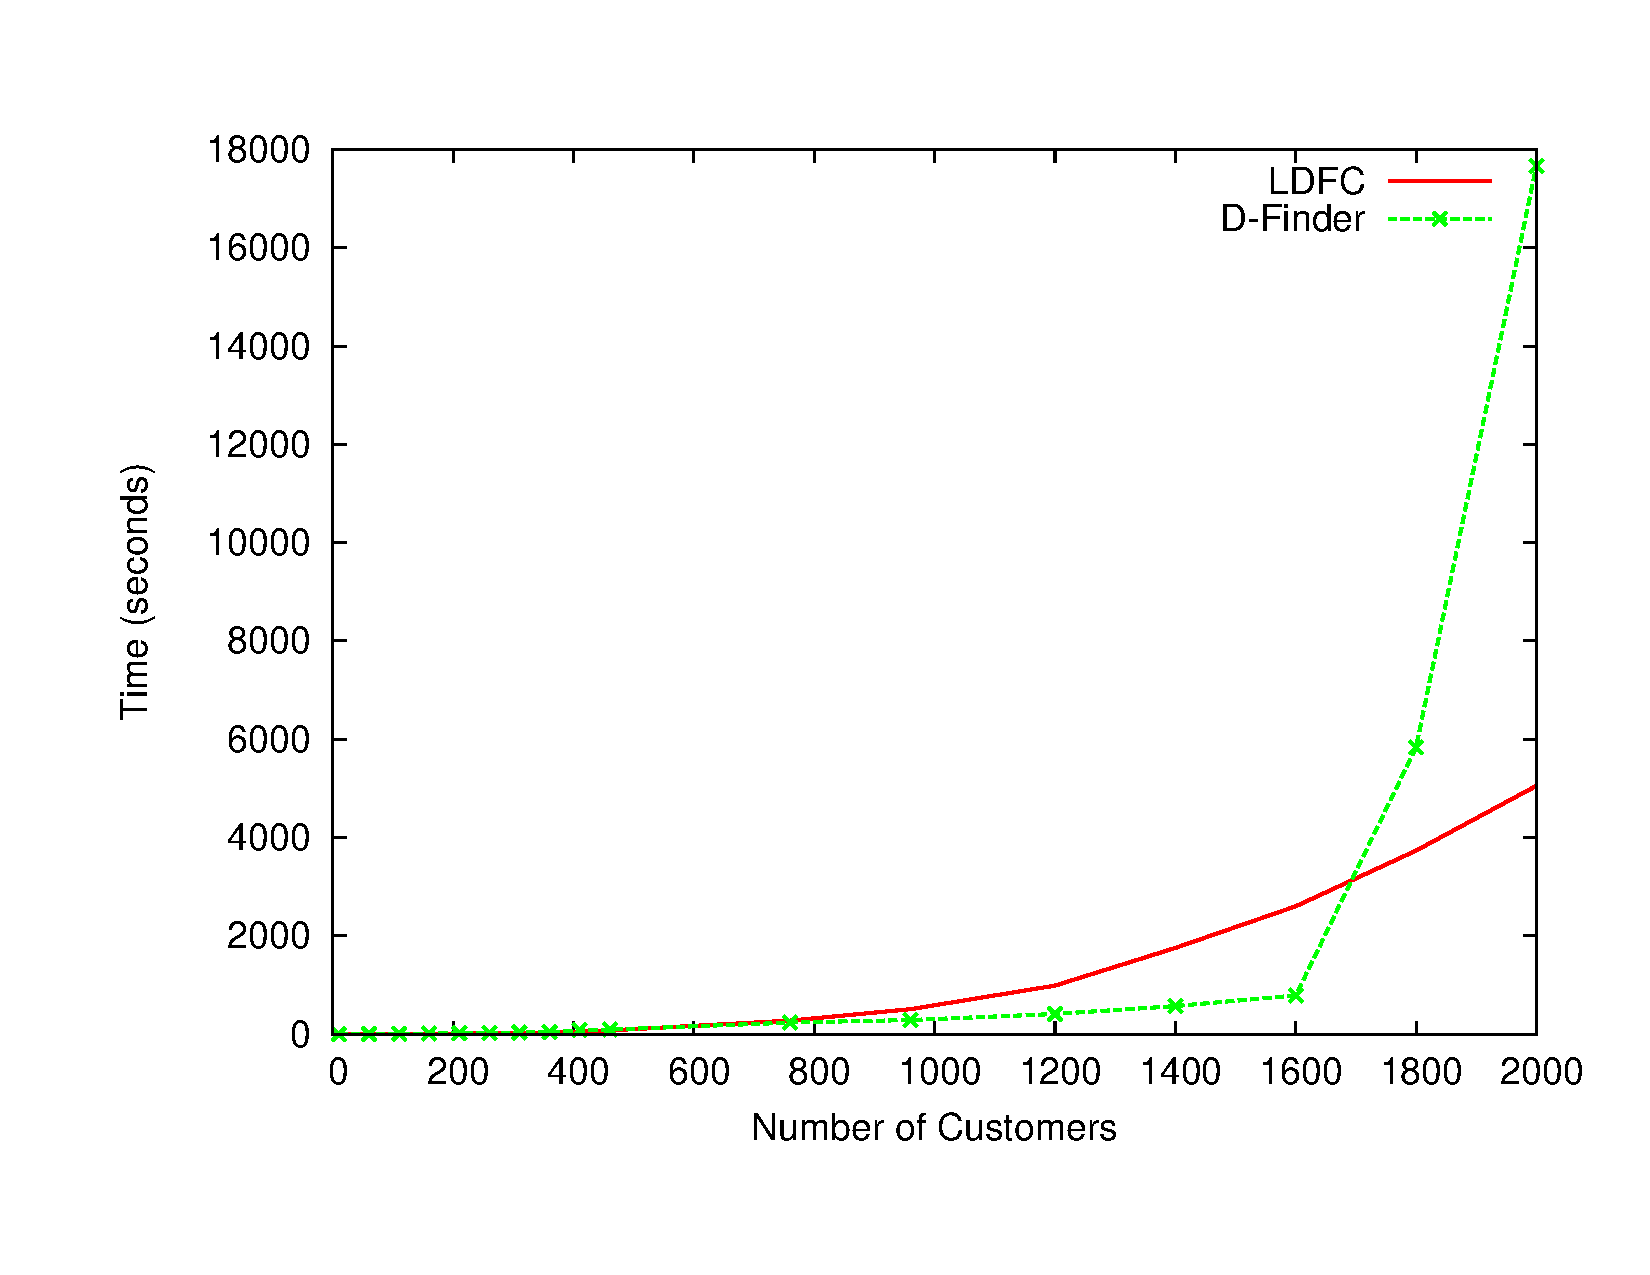
\includegraphics{figs/benchgas3.pdf}}}
      }\vspace*{-0.2cm}
    \caption{Benchmarks generated by our experiments.}
    \label{fig:gasSpectrum}
  \end{center}
\end{figure}




